%!TEX program = pdflatex
% Guide d'utilisation de l'espace conducteur de CamerRideShare.
% Compilation : latexmk -pdf guide-conducteur.tex   (deux passes pour la table des matières et les renvois)
% Les captures sont régénérées avec capture/capture-conducteur.mjs (voir README.md).
\documentclass[11pt,a4paper]{article}

\usepackage[utf8]{inputenc}
\usepackage[T1]{fontenc}
\usepackage[french]{babel}
\usepackage{helvet}
\renewcommand{\familydefault}{\sfdefault}
\usepackage[a4paper,left=2.3cm,right=2.3cm,top=2.6cm,bottom=2.4cm]{geometry}
\usepackage{xcolor}
\usepackage{graphicx}
\usepackage{float}
\usepackage{caption}
\usepackage{enumitem}
\usepackage{booktabs}
\usepackage{array}
\usepackage{tabularx}
\usepackage{fancyhdr}
\usepackage{titlesec}
\usepackage{tikz}
\usetikzlibrary{arrows.meta,positioning,shapes.geometric,calc,fit}
\usepackage[most]{tcolorbox}
\usepackage[hidelinks]{hyperref}
\usepackage{microtype}
\usepackage{etoolbox}
% Saut de page si la place restante est insuffisante (équivalent de needspace, sans extension supplémentaire)
\newcommand{\Needspace}[1]{\par\ifdim\pagegoal<\maxdimen\ifdim\dimexpr\pagegoal-\pagetotal\relax<#1\relax\newpage\fi\fi}
\AtBeginEnvironment{tabularx}{\setlength{\parskip}{0pt}}
\newcolumntype{L}[1]{>{\bfseries\raggedright\arraybackslash\textcolor{vert}\bgroup}p{#1}<{\egroup}}

% ─── Couleurs (celles de l'application) ──────────────────────────────────────
\definecolor{vert}{HTML}{148664}
\definecolor{vertclair}{HTML}{E4F3EE}
\definecolor{marque}{HTML}{E8590C}   % couleur des pastilles et des cadres sur les captures
\definecolor{marqueclair}{HTML}{FFF1E8}
\definecolor{bleu}{HTML}{1D4E89}
\definecolor{bleuclair}{HTML}{E8F0FA}
\definecolor{gris}{HTML}{5B6270}
\definecolor{grisclair}{HTML}{F3F4F6}
\definecolor{rouge}{HTML}{C62828}
\definecolor{rougeclair}{HTML}{FDECEC}

\hypersetup{pdftitle={Guide d'utilisation de l'espace conducteur -- CamerRideShare},pdfauthor={Abdoulrahim Momo Aboubakar}}

% ─── Pastille numérotée (identique à celles des captures) ────────────────────
\newcommand{\mk}[1]{\tikz[baseline=(c.base)]\node[circle,fill=marque,text=white,inner sep=0pt,minimum size=1.45ex+3pt,font=\bfseries\scriptsize\sffamily,draw=white,line width=0.4pt] (c) {#1};}

% Légende d'une capture : liste de pastilles expliquées
\newenvironment{legende}{\begin{list}{}{\setlength{\leftmargin}{2.1em}\setlength{\labelwidth}{1.8em}\setlength{\labelsep}{0.3em}\setlength{\itemsep}{2pt}\setlength{\topsep}{4pt}\setlength{\parsep}{0pt}\renewcommand{\makelabel}[1]{\hss##1}}}{\end{list}}

% Capture : \capture{fichier}{etiquette}{légende}{hauteur max en fraction de la page}
\newcommand{\capture}[4]{%
  \Needspace{\dimexpr#4\textheight+3.2cm\relax}
  \begin{figure}[H]\centering
  \fcolorbox{gris!45}{white}{\includegraphics[width=\linewidth,height=#4\textheight,keepaspectratio]{images/#1}}
  \caption{#3}\label{fig:#2}
  \end{figure}}

% Deux captures côte à côte (téléphone)
\newcommand{\captureduo}[5]{%
  \Needspace{\dimexpr#5\textheight+3.2cm\relax}
  \begin{figure}[H]\centering
  \fcolorbox{gris!45}{white}{\includegraphics[height=#5\textheight]{images/#1}}\hspace{1.2cm}%
  \fcolorbox{gris!45}{white}{\includegraphics[height=#5\textheight]{images/#2}}
  \caption{#4}\label{fig:#3}
  \end{figure}}

% ─── Encadrés ────────────────────────────────────────────────────────────────
\newtcolorbox{astuce}{enhanced,breakable,colback=vertclair,colframe=vert,boxrule=0.6pt,leftrule=3.5pt,arc=2pt,
  top=9pt,bottom=5pt,left=6pt,right=6pt,before skip=14pt,after skip=10pt,
  title={\textbf{Astuce}},coltitle=vert,colbacktitle=vertclair,fonttitle=\sffamily,attach boxed title to top left={yshift=-2.5mm,xshift=3mm},
  boxed title style={colback=white,colframe=vert,boxrule=0.5pt,arc=2pt,top=1pt,bottom=1pt}}
\newtcolorbox{attention}{enhanced,breakable,colback=rougeclair,colframe=rouge,boxrule=0.6pt,leftrule=3.5pt,arc=2pt,
  top=9pt,bottom=5pt,left=6pt,right=6pt,before skip=14pt,after skip=10pt,
  title={\textbf{Attention}},coltitle=rouge,colbacktitle=rougeclair,fonttitle=\sffamily,attach boxed title to top left={yshift=-2.5mm,xshift=3mm},
  boxed title style={colback=white,colframe=rouge,boxrule=0.5pt,arc=2pt,top=1pt,bottom=1pt}}
\newtcolorbox{retenir}{enhanced,breakable,colback=bleuclair,colframe=bleu,boxrule=0.6pt,leftrule=3.5pt,arc=2pt,
  top=9pt,bottom=5pt,left=6pt,right=6pt,before skip=14pt,after skip=10pt,
  title={\textbf{À retenir}},coltitle=bleu,colbacktitle=bleuclair,fonttitle=\sffamily,attach boxed title to top left={yshift=-2.5mm,xshift=3mm},
  boxed title style={colback=white,colframe=bleu,boxrule=0.5pt,arc=2pt,top=1pt,bottom=1pt}}

% Étapes numérotées
\setlist[enumerate,1]{label=\textbf{\textcolor{vert}{\arabic*.}},leftmargin=2em,itemsep=3pt,topsep=4pt}
\setlist[itemize,1]{leftmargin=1.6em,itemsep=2pt,topsep=4pt}
% Nom d'un bouton ou d'un menu, tel qu'il apparaît à l'écran
\newcommand{\bouton}[1]{\textbf{«\,#1\,»}}

% ─── Titres ──────────────────────────────────────────────────────────────────
\titleformat{\section}{\color{vert}\normalfont\sffamily\huge\bfseries}{\thesection}{0.6em}{}[\vspace{3pt}\color{vert}\titlerule]
\titleformat{\subsection}{\color{bleu}\normalfont\sffamily\Large\bfseries}{\thesubsection}{0.6em}{}
\titleformat{\subsubsection}{\color{gris}\normalfont\sffamily\large\bfseries}{}{0em}{}
\titlespacing*{\section}{0pt}{0pt}{14pt}
\titlespacing*{\subsection}{0pt}{16pt}{6pt}
\titlespacing*{\subsubsection}{0pt}{10pt}{3pt}
\captionsetup{font={small,sf},labelfont={bf,color=vert},labelsep=period,justification=centering,skip=6pt}

% Un titre de sous-section n'est jamais isolé en bas de page
\let\oldsubsection\subsection
\renewcommand{\subsection}{\Needspace{5.5cm}\oldsubsection}
% Chaque section (chapitre) commence sur une nouvelle page
\let\oldsection\section
\renewcommand{\section}{\clearpage\oldsection}

% ─── En-têtes ────────────────────────────────────────────────────────────────
\pagestyle{fancy}
\fancyhf{}
\renewcommand{\headrulewidth}{0.4pt}
\renewcommand{\footrulewidth}{0pt}
\fancyhead[L]{\small\color{gris}CamerRideShare -- Guide du conducteur}
\fancyhead[R]{\small\color{gris}\nouppercase{\leftmark}}
\fancyfoot[C]{\small\color{gris}Page \thepage}
\setlength{\headheight}{14pt}
\setlength{\parindent}{0pt}
\setlength{\parskip}{5pt plus 1pt}
\renewcommand{\arraystretch}{1.25}

\begin{document}

% ═══ PAGE DE GARDE ═══════════════════════════════════════════════════════════
\begin{titlepage}
\thispagestyle{empty}
\begin{tikzpicture}[remember picture,overlay]
  \fill[vert] (current page.north west) rectangle ([yshift=-11.2cm]current page.north east);
  \fill[marque] ([yshift=-11.2cm]current page.north west) rectangle ([yshift=-11.55cm]current page.north east);
  \node[anchor=north west,inner sep=0pt] at ([xshift=2.3cm,yshift=-2.2cm]current page.north west) {
\includegraphics[height=2.6cm]{images/logo.png}};
  \node[anchor=north west,text=white,align=left,inner sep=0pt] at ([xshift=2.3cm,yshift=-5.6cm]current page.north west)
    {{\sffamily\fontsize{34}{40}\selectfont\bfseries Guide d'utilisation}\\[6pt]{\sffamily\fontsize{22}{26}\selectfont Espace conducteur}};
  \node[anchor=north west,text=white,inner sep=0pt] at ([xshift=2.3cm,yshift=-9.4cm]current page.north west)
    {\sffamily\large CamerRideShare -- devenir propriétaire de son véhicule, semaine après semaine};
\end{tikzpicture}

\vspace*{10.2cm}

{\large Ce guide s'adresse à tout conducteur de moto-taxi ou de taxi, \textbf{sans aucune connaissance technique requise} : chaque écran est présenté pas à pas, avec des captures annotées. Le logiciel se lit très bien sur un téléphone.}

\vspace{1.2cm}
\begin{tcolorbox}[colback=grisclair,colframe=grisclair,arc=3pt,left=10pt,right=10pt,top=8pt,bottom=8pt]
\begin{tabularx}{\linewidth}{@{}L{3.2cm}X@{}}
Auteur & Abdoulrahim Momo Aboubakar\\
Version & 1.0 -- novembre 2026\\
Application & CamerRideShare, espace conducteur\\
Données & Les captures ont été réalisées avec des données fictives de démonstration.\\
\end{tabularx}
\end{tcolorbox}
\end{titlepage}

\tableofcontents
\clearpage

% ═══ AVANT-PROPOS ════════════════════════════════════════════════════════════
\section*{Comment utiliser ce guide}
\addcontentsline{toc}{section}{Comment utiliser ce guide}
\markboth{Comment utiliser ce guide}{Comment utiliser ce guide}

Ce guide vous accompagne de votre première connexion jusqu'à la gestion de vos paiements au quotidien. Vous n'avez pas besoin de le lire d'un trait : chaque chapitre correspond à une page du logiciel, et vous pouvez aller directement à celui dont vous avez besoin (voir aussi l'\hyperref[sec:taches]{index des tâches courantes} à la fin).

\subsection*{Les repères sur les captures d'écran}

Sur chaque capture, les zones importantes sont entourées d'un \textbf{cadre orange} et numérotées avec une \textbf{pastille orange} comme celle-ci : \mk{1}. Le texte situé sous la capture explique ce que chaque numéro désigne.

\subsection*{Les encadrés}

\begin{astuce}
Un conseil pour aller plus vite ou éviter une erreur courante.
\end{astuce}
\begin{attention}
Un point important, ou une action difficile à annuler : lisez-le avant de cliquer.
\end{attention}
\begin{retenir}
L'essentiel d'une notion, à garder en tête.
\end{retenir}

\subsection*{Les mots employés à l'écran}

Les noms entre guillemets, par exemple \bouton{Déclarer un paiement}, sont écrits exactement comme dans le logiciel : cherchez-les à l'écran. Le logiciel s'utilise avec la souris ou, sur téléphone et tablette, avec le doigt ; « cliquer » signifie aussi « toucher ». Tous les montants sont en \textbf{francs CFA} (FCFA ou XAF : c'est la même monnaie).

% ═══ 1. COMPRENDRE ═══════════════════════════════════════════════════════════
\section{Comprendre votre contrat}

\subsection{Le principe : devenir propriétaire}

CamerRideShare vous confie un véhicule. Chaque semaine, vous versez une somme fixe. Quand vous avez remboursé la totalité du \textbf{montant cible}, \textbf{le véhicule vous appartient}.

\begin{retenir}
Le montant cible est le total que vous remboursez, en versements hebdomadaires. Il comprend le prix d'achat du véhicule et la part des investisseurs qui l'ont financé. Vous ne payez jamais plus que ce total.
\end{retenir}

\subsection{Un exemple chiffré}

Prenons une moto dont le montant cible est de \textbf{880\,000~FCFA}, avec un versement de \textbf{27\,500~FCFA par semaine}.

\begin{center}
\begin{tabularx}{0.92\linewidth}{@{}Xr@{}}
\toprule
Montant cible à rembourser & 880\,000~FCFA\\
Versement chaque semaine & 27\,500~FCFA\\
Durée du contrat (880\,000 $\div$ 27\,500) & 32 semaines\\
Après 19 versements (522\,500~FCFA) : il vous reste à payer & 357\,500~FCFA\\
Votre part du véhicule à ce moment (522\,500 sur 880\,000) & 59\,\%\\
\bottomrule
\end{tabularx}
\end{center}

C'est exactement ce que vous voyez sur votre tableau de bord (voir \autoref{fig:dashboard}).

\subsection{Les règles à connaître}

\begin{center}
\begin{tabularx}{\linewidth}{@{}L{3.6cm}X@{}}
\toprule
Le versement & Vous versez le même montant chaque semaine, \textbf{avant dimanche soir}.\\
Le retard & Vous êtes en retard à partir du \textbf{lundi} qui suit une semaine non réglée.\\
Les conséquences & Le retard est signalé à l'administrateur, et \textbf{chaque semaine de retard ajoute une semaine} à la fin de votre calendrier. Rien n'est perdu : vous remboursez la même somme, un peu plus tard.\\
Verser plus & Si vous versez plus que le montant habituel, la dernière échéance est avancée d'autant.\\
Une panne & Les versements ne sont pas suspendus pendant une panne : signalez-la (voir \autoref{sec:support}).\\
\bottomrule
\end{tabularx}
\end{center}

\begin{astuce}
Un versement que vous avez \textbf{déclaré} compte déjà pour éviter le retard, même si l'administrateur ne l'a pas encore confirmé. Déclarez donc votre paiement le jour même.
\end{astuce}

\subsection{Les mots à connaître}

\begin{center}
\begin{tabularx}{\linewidth}{@{}L{3.6cm}X@{}}
\toprule
Montant cible & Ce que vous devez rembourser au total pour que le véhicule soit à vous.\\
Versement & La somme que vous payez chaque semaine.\\
Reste à payer & Le montant cible moins ce que vous avez déjà payé (versements \textbf{validés}).\\
Validé & L'administrateur a confirmé qu'il a bien reçu votre paiement.\\
En attente & Vous avez déclaré le paiement ; l'administrateur ne l'a pas encore confirmé.\\
Refusé & L'administrateur n'a pas accepté la déclaration (par exemple une preuve illisible). Vous en êtes prévenu, avec le motif.\\
Preuve de paiement & Une photo de votre reçu ou de la capture d'écran du transfert. Elle est facultative.\\
Signalement & Un message à l'administrateur pour l'informer d'un problème (panne, accident\ldots).\\
\bottomrule
\end{tabularx}
\end{center}

% ═══ 2. SE CONNECTER ═════════════════════════════════════════════════════════
\section{Se connecter et se repérer}

\subsection{Obtenir son accès}

On ne s'inscrit pas librement : c'est l'administrateur qui vous ouvre un compte. Il vous envoie par e-mail un \textbf{lien d'invitation} (valable sept jours) pour créer vous-même votre compte, ou bien il crée le compte pour vous et vous communique votre numéro de téléphone et un mot de passe provisoire. Dans les deux cas, \textbf{changez ce mot de passe} dès la première connexion (voir \autoref{sec:parametres}).

\subsection{Se connecter}

L'adresse du logiciel est celle que l'on vous a communiquée (par exemple \texttt{camerrideshare.strife-cyber.org}). Vous pouvez l'ouvrir dans n'importe quel navigateur, sur téléphone, tablette ou ordinateur.

\capture{01-connexion.png}{connexion}{La page de connexion.}{0.5}
\begin{legende}
  \item[\mk{1}] \textbf{Numéro de téléphone} : c'est votre identifiant. Saisissez-le sans espace, par exemple \texttt{690000011}.
  \item[\mk{2}] \textbf{Mot de passe}. Le petit œil, à droite, permet de l'afficher le temps de vérifier votre saisie.
  \item[\mk{3}] \textbf{Se connecter} : ouvre votre espace. Le bouton reste grisé tant que les deux champs ne sont pas remplis.
  \item[\mk{4}] Rappel : l'accès se fait \textbf{sur invitation}.
\end{legende}

\begin{attention}
Après plusieurs tentatives ratées, la connexion est bloquée quelques minutes par sécurité (dix essais sur quinze minutes). Patientez avant de réessayer. Ne communiquez jamais votre mot de passe : personne n'a besoin de vous le demander.
\end{attention}

\subsection{L'écran en un coup d'œil}

Toutes les pages de l'espace conducteur ont la même organisation.

\capture{02-reperes.png}{reperes}{Les zones communes à toutes les pages.}{0.5}
\begin{legende}
  \item[\mk{1}] \textbf{Le menu} : quatre entrées, une par page (tableau de bord, mes paiements, support, paramètres). La page affichée est surlignée en vert.
  \item[\mk{2}] \textbf{Le bouton de réduction} du menu : il le replie pour gagner de la place, ou le rouvre.
  \item[\mk{3}] \textbf{Le fil d'Ariane} : il rappelle où vous êtes.
  \item[\mk{4}] \textbf{La cloche} des notifications. Le chiffre indique combien de notifications sont non lues.
  \item[\mk{5}] \textbf{Le bouton lune} : bascule entre le thème clair et le thème sombre.
  \item[\mk{6}] \textbf{Votre profil} et le bouton \bouton{Déconnexion}. Pensez à vous déconnecter si le téléphone est partagé.
  \item[\mk{7}] \textbf{La zone de travail} : le contenu de la page choisie.
\end{legende}

\subsection{La cloche de notifications}

La cloche vous prévient de ce qui concerne votre contrat : un paiement enregistré, validé ou refusé, un véhicule qui vous est attribué ou retiré, un signalement traité, le rappel du vendredi\ldots

\capture{03-cloche.png}{cloche}{La liste des notifications.}{0.42}
\begin{legende}
  \item[\mk{1}] La cloche : cliquez dessus pour ouvrir la liste.
  \item[\mk{2}] \bouton{Tout lire} marque toutes les notifications comme lues.
  \item[\mk{3}] Une notification \textbf{non lue} est surlignée et précédée d'un point jaune. Cliquez dessus : elle est marquée comme lue et vous amène à la page concernée.
\end{legende}

La liste se met à jour toute seule environ toutes les trente secondes.

\subsection{Utiliser le logiciel sur téléphone}

Le logiciel s'adapte à l'écran du téléphone : le menu se range alors derrière un bouton.

\captureduo{21-mobile-a.png}{21-mobile-b.png}{mobile}{Sur téléphone : l'écran d'accueil (à gauche) et le menu ouvert (à droite).}{0.5}
\begin{legende}
  \item[\mk{1}] Le bouton qui \textbf{ouvre le menu}.
  \item[\mk{2}] La cloche de notifications.
  \item[\mk{3}] Le thème clair ou sombre.
  \item[\mk{4}] Le menu ouvert : touchez une entrée pour changer de page.
  \item[\mk{5}] Votre profil et la déconnexion.
  \item[\mk{6}] Touchez la zone grisée, à droite, pour fermer le menu.
\end{legende}

\subsection{Installer l'application sur l'écran d'accueil}

Vous pouvez installer CamerRideShare comme une vraie application, sans passer par un magasin d'applications. Elle s'ouvre alors en plein écran, avec son icône, et il suffit d'un doigt pour la lancer.

\subsubsection*{Sur téléphone Android ou sur ordinateur}

\capture{23-installation-bureau.png}{installbureau}{Le bouton d'installation, au-dessus de « Déconnexion ».}{0.2}
\begin{enumerate}
  \item Ouvrez le menu : si votre navigateur sait installer l'application, le bouton \mk{1} \bouton{Installer l'application} apparaît juste au-dessus de \mk{2} \bouton{Déconnexion}.
  \item Touchez-le et confirmez dans la fenêtre du navigateur.
\end{enumerate}

\subsubsection*{Sur iPhone ou iPad}

Apple n'affiche pas de fenêtre d'installation automatique : le bouton \bouton{Installer l'application} ouvre donc une petite explication.

\begin{figure}[H]\centering
\fcolorbox{gris!45}{white}{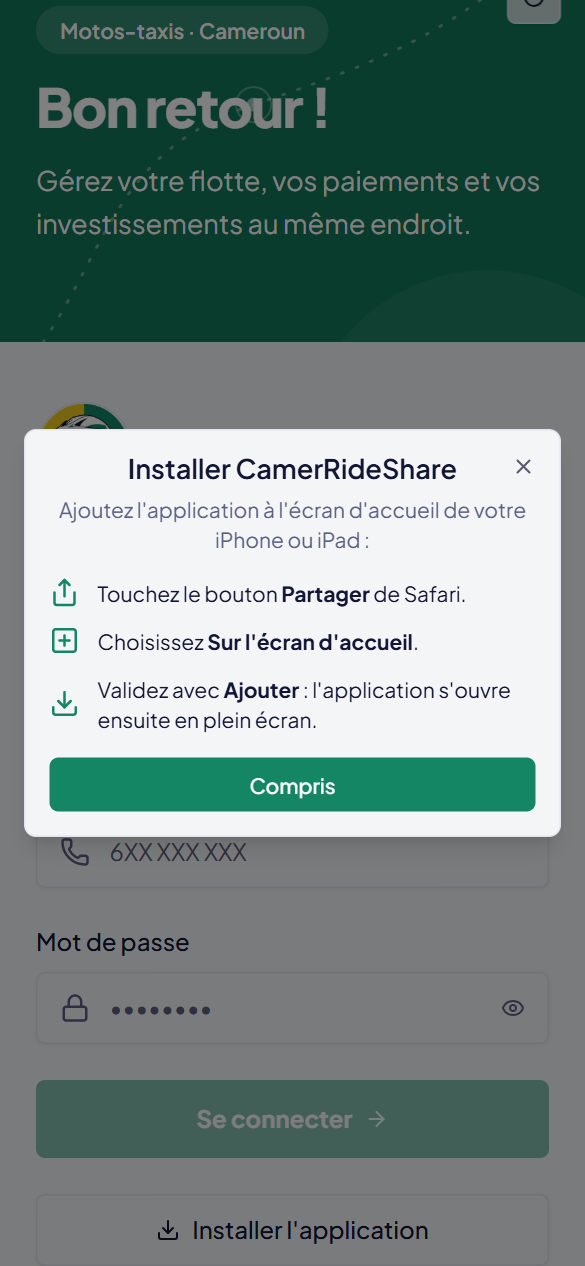
\includegraphics[height=0.42\textheight]{images/32-installation-iphone.png}}
\caption{Sur iPhone : la fenêtre d'explication.}\label{fig:iphone}
\end{figure}
\begin{enumerate}
  \item Ouvrez le logiciel dans \textbf{Safari}.
  \item Touchez le bouton \textbf{Partager} de Safari.
  \item Choisissez \bouton{Sur l'écran d'accueil}, puis \bouton{Ajouter}.
\end{enumerate}

\begin{astuce}
L'application installée \textbf{se met à jour toute seule} : à chaque nouvelle version, elle se renouvelle sans que vous ayez rien à faire. Si elle semble figée ou affiche un écran blanc, elle essaie de se réparer d'elle-même au bout de quelques secondes ; sinon, fermez-la complètement puis rouvrez-la.
\end{astuce}

% ═══ 3. TABLEAU DE BORD ══════════════════════════════════════════════════════
\section{Le tableau de bord}

C'est la page qui s'ouvre après la connexion. Elle répond à trois questions : \textit{où en suis-je ? combien me reste-t-il à payer ? suis-je à jour ?}

\capture{04-dashboard.png}{dashboard}{Le tableau de bord.}{0.75}
\begin{legende}
  \item[\mk{1}] \textbf{Progression} : le pourcentage du véhicule qui \textbf{vous appartient} (ici 59\,\%). Le vert est votre part ; le gris est ce qui reste à rembourser.
  \item[\mk{2}] \textbf{Reste à payer} : la somme qu'il vous reste à verser, et le pourcentage correspondant.
  \item[\mk{3}] \textbf{Mon contrat} : le bouton \bouton{Télécharger mon contrat (PDF)} (voir ci-dessous).
  \item[\mk{4}] \textbf{Statut} : êtes-vous à jour ou en retard ? Le bouton \bouton{Signaler un problème} est juste dessous.
  \item[\mk{5}] \textbf{Mes retards} : l'historique de vos retards, avec le nombre de semaines ajoutées à votre calendrier.
  \item[\mk{6}] \textbf{Paiements récents} : vos dix derniers versements, avec leur état.
\end{legende}

\subsection{Votre statut}

\capture{05-statut-retard.png}{statutretard}{Le tableau de bord d'un conducteur en retard.}{0.7}
\begin{legende}
  \item[\mk{1}] La carte \textbf{Statut}.
  \item[\mk{2}] Une pastille \textbf{En retard} (en rouge) remplace \textbf{À jour} (en vert).
  \item[\mk{3}] Le nombre de semaines de retard et la somme à régulariser (ici 3 semaines, 82\,500~FCFA). En dessous, le rappel de la date limite du versement de la semaine : \textit{avant dimanche soir}, avec le nombre de jours restants.
  \item[\mk{4}] La carte \textbf{Mes retards} : une ligne par semaine de retard, avec la date depuis laquelle vous êtes en retard et le nombre de jours.
  \item[\mk{5}] \textit{À régulariser} (rouge) : cette semaine n'est pas encore rattrapée.
  \item[\mk{6}] \textit{Régularisé} (vert) : vous avez rattrapé cette semaine. Elle reste dans l'historique.
\end{legende}

\begin{retenir}
Pour sortir du retard, \textbf{déclarez les versements manquants} (voir \autoref{sec:paiements}). Dès que l'administrateur les valide, le statut repasse à \textit{À jour}. Un versement déclaré compte déjà, même s'il est en attente.
\end{retenir}

\capture{06-retards-filtre.png}{retardsfiltre}{Filtrer l'historique des retards.}{0.2}
La liste déroulante \bouton{Tous les retards} permet de n'afficher que les retards \textit{à régulariser} ou ceux \textit{régularisés}.

\subsection{Télécharger votre contrat}

\capture{07-contrat-signaler.png}{contrat}{Le contrat et le signalement d'un problème.}{0.25}
\begin{enumerate}
  \item Touchez \mk{1} \bouton{Télécharger mon contrat (PDF)}.
  \item Le document est préparé en quelques secondes. Il contient votre véhicule, le montant à verser, le versement hebdomadaire et le calendrier des échéances. Conservez-le.
\end{enumerate}

\subsection{Signaler un problème depuis le tableau de bord}

Le bouton \mk{2} \bouton{Signaler un problème} ouvre une petite fenêtre pour prévenir l'administrateur tout de suite.

\capture{08-signaler-modale.png}{signalermodale}{La fenêtre de signalement rapide.}{0.25}
\begin{enumerate}
  \item \mk{1} Décrivez le problème en quelques mots.
  \item \mk{3} Touchez \bouton{Envoyer}. \mk{2} \bouton{Annuler} ferme la fenêtre sans rien envoyer.
\end{enumerate}

Pour un signalement plus complet (catégorie, photo), utilisez la page \bouton{Support} (voir \autoref{sec:support}).

% ═══ 4. MES PAIEMENTS ════════════════════════════════════════════════════════
\section{Mes paiements}\label{sec:paiements}

Cette page est celle que vous utiliserez le plus souvent : vous y \textbf{déclarez} vos versements et vous suivez tout votre historique.

\capture{09-paiements.png}{paiements}{La page « Mes paiements ».}{0.75}
\begin{legende}
  \item[\mk{1}] \bouton{Déclarer un paiement} (voir \autoref{fig:declarer}).
  \item[\mk{2}] \textbf{Total payé} : la somme de vos versements \textbf{validés}. En dessous, ce qui est \textit{en attente de validation}.
  \item[\mk{3}] \textbf{Reste à payer}, sur le total à rembourser. \mk{4} \textbf{Dernier versement} : montant et date.
  \item[\mk{5}] La \textbf{recherche} : tapez un montant exact pour retrouver un versement. \mk{6} Le filtre de \textbf{statut} et \mk{7} le filtre de \textbf{moyen de paiement}.
  \item[\mk{8}] \textbf{Preuve} : le lien \bouton{Voir} ouvre la photo de la preuve de paiement jointe (un tiret signifie qu'il n'y en a pas).
  \item[\mk{9}] Le \textbf{statut} : \textit{En attente}, \textit{Validé} ou \textit{Refusé}.
  \item[\mk{10}] La \textbf{corbeille} : elle n'apparaît que sur un paiement \textit{en attente}, pour le retirer en cas d'erreur.
\end{legende}

Le tableau s'affiche dix lignes par dix lignes : utilisez \bouton{Précédent} et \bouton{Suivant} en bas de la liste. Une ligne \textit{Dépense} est une somme saisie par l'administrateur pour votre compte.

\subsection{Déclarer un paiement}

Déclarez votre versement \textbf{dès que vous l'avez effectué} (Orange Money, MTN Money, ou espèces remises à l'administrateur).

\capture{10-declarer.png}{declarer}{La fenêtre « Déclarer un paiement ».}{0.5}
\begin{enumerate}
  \item Touchez \bouton{Déclarer un paiement}.
  \item \mk{1} Saisissez le \textbf{montant} en francs CFA, sans espace. Le champ est prérempli avec le versement de la semaine (27\,500~FCFA ici). Vous ne pouvez pas dépasser ce qui vous reste à payer.
  \item \mk{2} Choisissez le \textbf{moyen de paiement} : \textit{Orange Money}, \textit{MTN Money} ou \textit{Espèces}.
  \item \mk{3} Si vous le pouvez, ajoutez la \textbf{preuve de paiement} (facultatif) : \bouton{Prendre une photo} utilise la caméra du téléphone, \bouton{Importer une image} choisit une photo déjà enregistrée. Formats : JPEG, PNG ou WebP, 5~Mo au plus.
  \item \mk{4} Touchez \bouton{Envoyer}.
\end{enumerate}

Votre paiement apparaît alors dans la liste avec le statut \textit{En attente}. L'administrateur est prévenu.

\begin{astuce}
Pour un paiement Orange Money ou MTN Money, \textbf{joignez la capture d'écran du message de confirmation} : l'administrateur peut ainsi valider plus vite. Pour de l'argent liquide, la preuve n'est généralement pas nécessaire.
\end{astuce}

\begin{figure}[H]\centering
\fcolorbox{gris!45}{white}{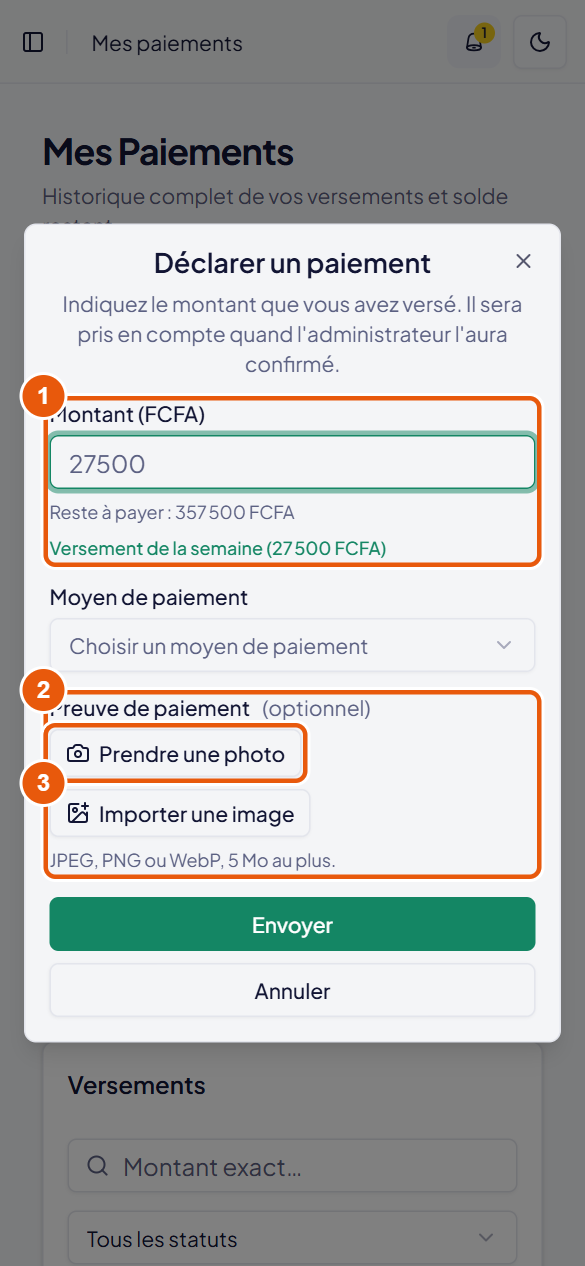
\includegraphics[height=0.42\textheight]{images/22-mobile-paiement.png}}
\caption{La même fenêtre sur téléphone.}\label{fig:mobilepaiement}
\end{figure}

\subsection{Ce qui se passe ensuite}

\begin{center}
\begin{tabularx}{\linewidth}{@{}L{3.2cm}X@{}}
\toprule
Validé & L'administrateur a confirmé la réception : la somme est retirée de votre \textit{reste à payer}. Vous recevez une notification.\\
Refusé & L'administrateur n'a pas accepté la déclaration. Vous recevez une notification avec le \textbf{motif} (par exemple « preuve illisible »). Déclarez de nouveau votre paiement en corrigeant le problème, par exemple avec une photo plus nette.\\
Toujours en attente & Pas d'inquiétude : tant que l'administrateur ne s'est pas prononcé, le paiement compte déjà pour éviter le retard.\\
\bottomrule
\end{tabularx}
\end{center}

\subsection{Retrouver un paiement}

\capture{11-statuts.png}{filtres}{Filtrer par statut.}{0.16}
Le filtre de statut propose \mk{1} \bouton{Validés}, \mk{2} \bouton{En attente} et \mk{3} \bouton{Refusés}. Le filtre de moyen propose \bouton{Orange Money}, \bouton{MTN Money} et \bouton{Espèces}. Vous pouvez aussi saisir un \textbf{montant exact} dans la recherche.

\subsection{Retirer un paiement déclaré par erreur}

Tant qu'un paiement est \textit{en attente}, vous pouvez le retirer avec la corbeille. C'est utile, par exemple, si vous avez saisi un mauvais montant.

\capture{12-retirer.png}{retirer}{La confirmation avant de retirer un paiement en attente.}{0.25}
\begin{enumerate}
  \item Touchez la corbeille sur la ligne du paiement en attente.
  \item Lisez la question : \textit{Retirer ce paiement en attente ?}
  \item \mk{2} Touchez \bouton{Retirer} pour confirmer, ou \mk{1} \bouton{Annuler} pour renoncer.
\end{enumerate}

\begin{attention}
Retirer un paiement est \textbf{irréversible}. Ne le faites que pour une erreur de saisie. Une fois le paiement validé ou refusé, il ne peut plus être retiré. Si vous avez retiré un paiement par erreur, déclarez-le de nouveau.
\end{attention}

% ═══ 5. SUPPORT ══════════════════════════════════════════════════════════════
\section{Le support}\label{sec:support}

La page \bouton{Support} réunit les réponses à vos questions, les moyens de joindre l'équipe et le formulaire pour signaler un problème.

\capture{13-support.png}{support}{La page « Support ».}{0.7}
\begin{legende}
  \item[\mk{1}] \textbf{Foire aux questions} : des réponses aux questions les plus courantes. Elles reprennent \textbf{vos vraies données} (votre versement, votre montant cible\ldots).
  \item[\mk{2}] \textbf{Contact direct} : les horaires de l'équipe, un bouton \bouton{WhatsApp Support}, un bouton pour \bouton{Appeler} (sur téléphone, il lance l'appel) et \bouton{Copier le numéro}.
  \item[\mk{3}] \textbf{Signaler un problème} : le formulaire (voir ci-dessous).
  \item[\mk{4}] \textbf{Mes signalements} : le suivi de vos signalements.
\end{legende}

\subsection{La foire aux questions}

\capture{14-faq.png}{faq}{Une question ouverte dans la foire aux questions.}{0.3}
\begin{enumerate}
  \item \mk{1} Tapez quelques mots dans la \textbf{recherche} pour retrouver une question.
  \item \mk{2} Touchez une question pour afficher la réponse ; touchez-la de nouveau pour la refermer.
\end{enumerate}

Six questions sont proposées : comment déclarer un versement, que se passe-t-il en cas de retard, que faire en cas de panne ou d'accident, quand la moto vous appartient, où télécharger le contrat et comment changer le mot de passe.

\subsection{Signaler un problème}

Utilisez ce formulaire pour une \textbf{panne}, un \textbf{accident}, un \textbf{vol}, ou toute autre difficulté. L'administrateur est prévenu \textbf{tout de suite}, et le signalement est automatiquement rattaché à votre véhicule.

\capture{15-signalement.png}{signalement}{Le formulaire « Signaler un problème ».}{0.45}
\begin{enumerate}
  \item \mk{1} Choisissez la \textbf{catégorie}.
  \item \mk{2} Décrivez la situation (\textbf{10 caractères minimum}, 1\,000 au plus). Un compteur vous indique ce qu'il reste à écrire.
  \item \mk{3} Ajoutez une \textbf{photo} si cela aide (facultatif) : \bouton{Prendre une photo} ou \bouton{Importer une image} (JPEG, PNG ou WebP, 5~Mo au plus).
  \item \mk{4} Touchez \bouton{Envoyer le signalement}. Le bouton reste grisé tant que la catégorie et la description ne sont pas valides.
\end{enumerate}

\capture{16-categories.png}{categories}{Les quatre catégories de signalement.}{0.18}
Les catégories sont : \bouton{Panne mécanique}, \bouton{Accident}, \bouton{Retard de paiement} et \bouton{Autre}.

\begin{attention}
En cas d'accident grave ou de danger immédiat, \textbf{appelez d'abord les secours}, puis l'administrateur. Le signalement ne remplace pas un appel.
\end{attention}

\subsection{Suivre vos signalements}

\capture{17-signalements.png}{signalements}{Le suivi de vos signalements.}{0.35}
\begin{legende}
  \item[\mk{1}] \textit{En cours de traitement} : l'administrateur a reçu votre message et s'en occupe.
  \item[\mk{2}] \textit{Photo jointe} : vous avez envoyé une photo avec ce signalement.
  \item[\mk{3}] \textit{Résolu} : l'administrateur a clos le signalement. La date est indiquée, et vous recevez une notification.
\end{legende}

% ═══ 6. PARAMÈTRES ═══════════════════════════════════════════════════════════
\section{Les paramètres}\label{sec:parametres}

La page \bouton{Paramètres} regroupe trois onglets. Les modifications ne sont \textbf{enregistrées} que lorsque vous touchez \bouton{Enregistrer les modifications}, dans la barre du bas ; \bouton{Réinitialiser} annule ce que vous venez de saisir.

\subsection{Profil}

\capture{18-parametres-profil.png}{profil}{L'onglet « Profil ».}{0.5}
\begin{legende}
  \item[\mk{1}] Les trois onglets : \bouton{Profil}, \bouton{Notifications} et \bouton{Compte}.
  \item[\mk{2}] Votre \textbf{photo} : \bouton{Prendre une photo} utilise la caméra ; \bouton{importer une image} choisit un fichier.
  \item[\mk{3}] Votre \textbf{nom complet}, qui figure sur votre contrat.
  \item[\mk{4}] Votre \textbf{numéro de téléphone}, qui sert aussi d'\textbf{identifiant de connexion}.
  \item[\mk{5}] Votre \textbf{adresse e-mail} : elle reçoit les messages de la plateforme, par exemple vos nouveaux identifiants si l'administrateur les réinitialise.
  \item[\mk{6}] \bouton{Modifier} permet de changer votre mot de passe. Pour votre sécurité, le mot de passe n'est jamais affiché.
  \item[\mk{7}] \bouton{Enregistrer les modifications}.
\end{legende}

\subsubsection*{Changer son mot de passe}
\begin{enumerate}
  \item Touchez \mk{6} \bouton{Modifier}.
  \item Saisissez votre \textbf{mot de passe actuel}, puis le \textbf{nouveau} (6 caractères minimum).
  \item Enregistrez.
\end{enumerate}

\begin{astuce}
Choisissez un mot de passe que vous n'utilisez nulle part ailleurs, et changez celui qui vous a été communiqué à la création de votre compte.
\end{astuce}

\subsection{Notifications}

\capture{19-parametres-notifications.png}{notifs}{L'onglet « Notifications ».}{0.4}
\begin{legende}
  \item[\mk{1}] \textbf{Suivi de mes paiements} : une notification quand un versement est enregistré, validé, refusé ou remis en attente par l'administrateur.
  \item[\mk{2}] \textbf{Rappel de versement} : chaque \textbf{vendredi matin}, un rappel dans l'application tant que le versement de la semaine n'est pas réglé, avec le montant restant à verser.
  \item[\mk{3}] Certaines notifications sont \textbf{toujours envoyées}, car elles engagent votre contrat : véhicule affecté ou retiré, résiliation, signalement traité.
\end{legende}

\begin{astuce}
Laissez le rappel du vendredi activé : c'est le meilleur moyen de ne jamais oublier un versement.
\end{astuce}

\subsection{Compte}

\capture{20-parametres-compte.png}{compte}{L'onglet « Compte ».}{0.4}
\begin{legende}
  \item[\mk{1}] Les informations de votre compte, \textbf{en lecture seule} : la date d'inscription, votre véhicule et la date à laquelle il vous a été affecté.
  \item[\mk{2}] \textbf{Thème sombre} : réglage propre à cet appareil.
  \item[\mk{3}] \bouton{Se déconnecter}.
\end{legende}

% ═══ 7. ROUTINE ══════════════════════════════════════════════════════════════
\section{Votre routine de conducteur}

\subsection{Chaque semaine}
\begin{enumerate}
  \item \textbf{Avant dimanche soir}, effectuez votre versement (Orange Money, MTN Money ou espèces).
  \item Dès que c'est fait, ouvrez \bouton{Mes paiements} et \bouton{Déclarer un paiement}, avec la preuve si vous en avez une.
  \item Vérifiez sur le \textbf{tableau de bord} que votre statut est \textit{À jour}.
\end{enumerate}

\subsection{Dès qu'il y a un problème}
\begin{enumerate}
  \item \bouton{Signaler un problème} (tableau de bord ou page \bouton{Support}).
  \item Suivez le traitement dans \bouton{Mes signalements}.
\end{enumerate}

\subsection{De temps en temps}
\begin{enumerate}
  \item Regardez votre \textbf{progression} : c'est la part du véhicule qui est à vous.
  \item Téléchargez votre \textbf{contrat} et gardez-le avec vous.
  \item Vérifiez que votre \textbf{numéro de téléphone} et votre \textbf{adresse e-mail} sont à jour.
\end{enumerate}

\subsection{Quelques bonnes pratiques}
\begin{itemize}
  \item \textbf{Ne partagez jamais} votre mot de passe, et déconnectez-vous d'un téléphone partagé.
  \item \textbf{Déclarez chaque versement le jour même} : un paiement déclaré protège du retard.
  \item \textbf{Gardez vos reçus} (messages Orange Money et MTN Money) jusqu'à la validation.
  \item Ne remettez jamais d'argent liquide sans que \textbf{l'administrateur le confirme} dans le logiciel.
\end{itemize}

% ═══ 8. DÉPANNAGE ════════════════════════════════════════════════════════════
\section{Que faire si\ldots}

\begin{center}
\begin{tabularx}{\linewidth}{@{}>{\bfseries\raggedright}p{4.4cm}X@{}}
\toprule
Je n'arrive pas à me connecter & Vérifiez le numéro (sans espaces) et le mot de passe. Après plusieurs essais ratés, attendez quelques minutes. Si vous avez oublié votre mot de passe, contactez l'administrateur : il peut le réinitialiser.\\
\midrule
Mon paiement est resté « en attente » & C'est normal tant que l'administrateur ne l'a pas vérifié. Il compte déjà pour éviter le retard. Si l'attente est longue, contactez le support (WhatsApp ou téléphone).\\
\midrule
Mon paiement a été refusé & Lisez le motif dans la notification. Corrigez le problème (par exemple une photo plus nette) et déclarez de nouveau le paiement.\\
\midrule
J'ai déclaré un mauvais montant & Si le paiement est encore \textit{en attente}, retirez-le avec la corbeille et déclarez-le de nouveau. S'il est déjà validé, contactez l'administrateur.\\
\midrule
Je suis en retard & Déclarez les versements manquants dès que possible. Chaque semaine de retard ajoute une semaine à la fin de votre calendrier, mais vous ne payez pas plus au total.\\
\midrule
Mon véhicule est en panne & Faites un signalement (catégorie \textit{Panne mécanique}) et prévenez l'administrateur. Les versements ne sont pas suspendus : signalez aussi tout retard.\\
\midrule
Je veux mon contrat & Tableau de bord, carte \bouton{Mon contrat}, bouton \bouton{Télécharger mon contrat (PDF)}.\\
\midrule
Je ne reçois pas les messages & Vérifiez l'adresse e-mail de votre profil et regardez dans vos courriers indésirables. Les notifications de l'application restent visibles dans la cloche.\\
\midrule
Le logiciel affiche une erreur ou reste bloqué & Actualisez la page. Sur l'application installée, fermez-la complètement puis rouvrez-la : elle se met à jour et se répare seule. Une bannière vous prévient aussi si votre connexion Internet est coupée.\\
\bottomrule
\end{tabularx}
\end{center}

% ═══ INDEX DES TÂCHES ════════════════════════════════════════════════════════
\section{Index des tâches courantes}\label{sec:taches}

\begin{center}
\begin{tabularx}{\linewidth}{@{}Xr@{}}
\toprule
\textbf{Je veux\ldots} & \textbf{Page}\\
\midrule
me connecter, installer l'application & \pageref{fig:connexion}\\
savoir combien il me reste à payer & \pageref{fig:dashboard}\\
voir si je suis en retard & \pageref{fig:statutretard}\\
télécharger mon contrat & \pageref{fig:contrat}\\
déclarer un paiement & \pageref{fig:declarer}\\
voir l'historique de mes paiements & \pageref{fig:paiements}\\
retirer un paiement déclaré par erreur & \pageref{fig:retirer}\\
signaler une panne ou un accident & \pageref{fig:signalement}\\
suivre un signalement & \pageref{fig:signalements}\\
joindre le support (WhatsApp, téléphone) & \pageref{fig:support}\\
changer mon mot de passe ou ma photo & \pageref{fig:profil}\\
choisir mes notifications & \pageref{fig:notifs}\\
\bottomrule
\end{tabularx}
\end{center}

\vfill
\begin{center}\small\color{gris}
Guide rédigé par Abdoulrahim Momo Aboubakar -- CamerRideShare, novembre 2026.\\
Les captures d'écran présentent des données fictives de démonstration.
\end{center}

\end{document}
